% !TEX program = xelatex
% This xelatex template is made by Milvoid
% NOT ALL THE CONTENTS ARE MADE BY Tuo Yao (Emptope)
% Copyleft 2026 Tuo Yao (Emptope), All wrongs reversed.
% Pasteright 6202 Xiran Wang, Nothing rights deserved.

\documentclass[a4paper]{article}

% Package loading
\usepackage{iftex}
\ifXeTeX
\else
  \errmessage{CheatSheet.tex must be compiled with XeLaTeX}
\fi

\usepackage[
  a4paper,
  left=0.10cm,
  right=0.10cm,
  top=0.10cm,
  bottom=0.25cm,
  noheadfoot
]{geometry}
\usepackage[no-math]{fontspec}
\usepackage{xeCJK}
\usepackage{xcolor}
\usepackage{multicol}
\usepackage{titlesec}
\usepackage{enumitem}
\usepackage{amssymb}
\usepackage{mathtools}
\usepackage{array}
\usepackage{booktabs}
\usepackage{tabularx}

% Font setup
\newcommand{\CheatFontPath}{fonts/}
\IfFileExists{fonts/SFCompactText-Regular.ttf}{}
  {\renewcommand{\CheatFontPath}{CheatSheetTemplate/fonts/}}

\defaultfontfeatures{Ligatures=TeX}
\defaultfontfeatures[SFCompactText-Regular.ttf]{
  Path=\CheatFontPath,
  BoldFont=SFCompactText-Bold.ttf,
  ItalicFont=SFCompactText-Italic.ttf,
  BoldItalicFont=SFCompactText-BoldItalic.ttf
}
\defaultfontfeatures[PingFangSC-Regular.ttf]{
  Path=\CheatFontPath,
  BoldFont=PingFangSC-SemiBold.ttf,
  ItalicFont=PingFangSC-Regular.ttf
}
\defaultfontfeatures[
  SFCompactText-SemiBold.ttf, SFCompactText-SemiBlack.ttf,
  PingFangSC-SemiBold.ttf, PingFangSC-SemiBlack.ttf
]{Path=\CheatFontPath}

\setmainfont{SFCompactText-Regular.ttf}
\setsansfont{SFCompactText-Regular.ttf}
\setmonofont{SFCompactText-Regular.ttf}

\setCJKmainfont{PingFangSC-Regular.ttf}
\setCJKsansfont{PingFangSC-Regular.ttf}
\setCJKmonofont{PingFangSC-Regular.ttf}

\newfontfamily\CheatLatinSemiBold{SFCompactText-SemiBold.ttf}
\newfontfamily\CheatLatinSemiBlack{SFCompactText-SemiBlack.ttf}
\newCJKfontfamily\CheatCJKSemiBold{PingFangSC-SemiBold.ttf}
\newCJKfontfamily\CheatCJKSemiBlack{PingFangSC-SemiBlack.ttf}

\xeCJKsetup{
  CJKmath=true,
  CheckSingle=true,
  PunctStyle=kaiming
}

% Math font setup
\DeclareFontFamily{OT1}{CheatMathRoman}{}
\DeclareFontShape{OT1}{CheatMathRoman}{m}{n}{<-> cmr10}{}
\DeclareFontFamily{OML}{CheatMathItalic}{\skewchar\font=127}
\DeclareFontShape{OML}{CheatMathItalic}{m}{it}{<-> cmmi10}{}
\DeclareFontFamily{OMS}{CheatMathSymbol}{\skewchar\font=48}
\DeclareFontShape{OMS}{CheatMathSymbol}{m}{n}{<-> cmsy10}{}
\DeclareFontFamily{OMX}{CheatMathLargeSymbol}{}
\DeclareFontShape{OMX}{CheatMathLargeSymbol}{m}{n}{<-> cmex10}{}

\SetSymbolFont{operators}{normal}{OT1}{CheatMathRoman}{m}{n}
\SetSymbolFont{letters}{normal}{OML}{CheatMathItalic}{m}{it}
\SetSymbolFont{symbols}{normal}{OMS}{CheatMathSymbol}{m}{n}
\SetSymbolFont{largesymbols}{normal}{OMX}{CheatMathLargeSymbol}{m}{n}

\newcommand{\CheatInlineMathSize}{5}
\newcommand{\CheatInlineMathScriptSize}{4.2}
\newcommand{\CheatInlineMathScriptScriptSize}{3.3}
\DeclareMathSizes
  {5} % must be the same as text size
  {\CheatInlineMathSize}
  {\CheatInlineMathScriptSize}
  {\CheatInlineMathScriptScriptSize}

\newcommand{\CheatInlineMathFont}{%
  \fontsize{\CheatInlineMathSize pt}{6pt}\selectfont
}
\everymath\expandafter{\expandafter\CheatInlineMathFont\the\everymath}

\thinmuskip=3mu
\medmuskip=4mu plus 2mu minus 4mu
\thickmuskip=5mu plus 5mu

% Page and column setup
\newlength{\CheatColumnWidth}
\newlength{\CheatColumnSep}
\newlength{\CheatTextWidth}
\setlength{\CheatColumnWidth}{5.07cm}
\setlength{\CheatColumnSep}{0.2cm}
\setlength{\CheatTextWidth}{\dimexpr 4\CheatColumnWidth + 3\CheatColumnSep\relax}
\setlength{\textwidth}{\CheatTextWidth}
\setlength{\columnsep}{\CheatColumnSep}
\setlength{\columnseprule}{0pt}
\setlength{\parindent}{0pt}
\setlength{\parskip}{0pt}
\setlength{\topskip}{0pt}
\setlength{\partopsep}{0pt}
\pagestyle{empty}

% Typography and colors
\definecolor{CheatTitleBlue}{HTML}{004D80}
\definecolor{CheatAccentBlue}{HTML}{0076BA}
\definecolor{CheatDividerGray}{HTML}{808080}

\makeatletter
\renewcommand\normalsize{%
  \@setfontsize\normalsize{5pt}{6pt}%
  \abovedisplayskip 1pt plus 0.5pt minus 0.5pt%
  \belowdisplayskip 1pt plus 0.5pt minus 0.5pt%
  \abovedisplayshortskip 0.5pt plus 0.5pt%
  \belowdisplayshortskip 0.5pt plus 0.5pt%
}
\makeatother
\normalsize

\titleformat{\section}
  {\color{CheatTitleBlue}\fontsize{7pt}{7.5pt}\selectfont}
  {}{0pt}{}
\titleformat{\subsection}
  {\color{CheatTitleBlue}\fontsize{6pt}{6.5pt}\selectfont\CheatLatinSemiBold\CheatCJKSemiBold}
  {}{0pt}{}
\titlespacing*{\section}{0pt}{1.2pt}{0.6pt}
\titlespacing*{\subsection}{0pt}{0.9pt}{0.4pt}
\setcounter{secnumdepth}{0}

\setlist[itemize]{
  leftmargin=0.85em,
  label={-},
  labelsep=0.25em,
  itemsep=0pt,
  topsep=0pt,
  parsep=0pt,
  partopsep=0pt
}
\setlist[enumerate]{
  leftmargin=1.1em,
  labelsep=0.25em,
  itemsep=0pt,
  topsep=0pt,
  parsep=0pt,
  partopsep=0pt
}
\renewcommand{\arraystretch}{0.95}
\setlength{\tabcolsep}{1.5pt}
\allowdisplaybreaks
\raggedright
\emergencystretch=0.8em
% Document-level commands and environments
\newenvironment{cheatsheet}
  {\begin{multicols*}{4}\raggedcolumns\normalsize}
  {\end{multicols*}}

\newcommand{\bluebf}[1]{\textcolor{CheatTitleBlue}{\textbf{#1}}}
\newcommand{\term}[1]{\textbf{#1}}
\newcommand{\accenttext}[1]{{\color{CheatAccentBlue}#1}}

\newcommand{\pointtitle}[1]{{\color{CheatAccentBlue}\CheatLatinSemiBlack\CheatCJKSemiBlack #1}}
\newcommand{\pt}[1]{\pointtitle{#1}}
\newcommand{\paragraphtitle}[1]{\pointtitle{#1}}
\newcommand{\bullettitle}[1]{\pointtitle{#1}}

\newcommand{\divider}{%
  \par\vspace{1pt}%
  {\color{CheatDividerGray}\hrule height 0.5pt width \linewidth}%
  \vspace{1pt}%
}

\newcommand{\m}[1]{{\CheatInlineMathFont\(#1\)}}
\newcommand{\tightmath}[1]{\m{#1}}
\newcommand{\diff}{\mathop{}\!\mathrm{d}}

\begin{document}
\begin{cheatsheet}

\section{这是大标题}

\divider

\section{这也是大标题}

\subsection{这是小标题}

更小的标题可以通过 \verb|\bluebf{}| 来强调：

\bluebf{这是更小的标题}

\divider

\subsection{公式示例}

行内公式：\m{\mathrm{e}^{\mathrm{i} \mathrm{\pi}} + 1 = 0}

行间公式：$$\mathrm{e}^{\mathrm{i} \mathrm{\pi}} + 1 = 0$$

\vspace{0.5em}

\subsection{插入图片示例}

单幅图片：

{\centering
 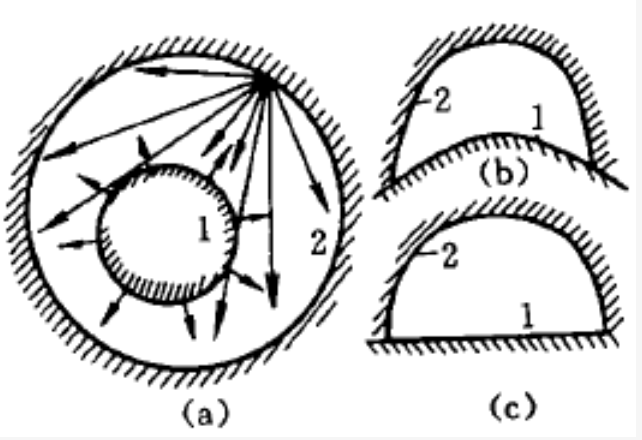
\includegraphics[height=1cm, width=0.3\linewidth]{fig/1.png}\par
}

多幅图片：

{\centering
 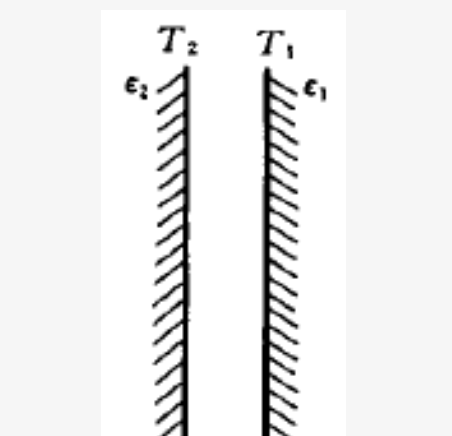
\includegraphics[height=1cm, width=0.3\linewidth]{fig/2.png}
 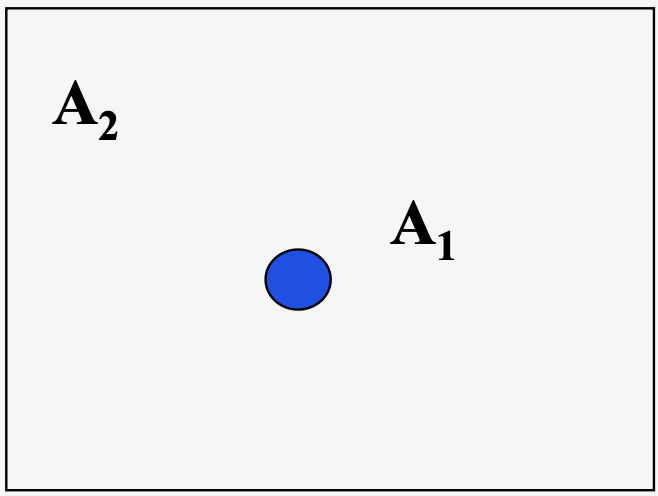
\includegraphics[height=1cm, width=0.3\linewidth]{fig/3.png}\par
}

\vspace{0.5em}

\divider

\subsection{表格示例}

\begingroup
\fontsize{4pt}{4.8pt}\selectfont
\setlength{\tabcolsep}{0.9pt}
\renewcommand{\arraystretch}{1.08}
\begin{tabularx}{\linewidth}{
  >{\raggedright\arraybackslash}p{0.31\linewidth}
  >{\raggedright\arraybackslash}X
  >{\raggedright\arraybackslash}X
}
\toprule
\term{检验类型} & \term{备择假设} & \term{临界值($\alpha=0.05$)} \\
\midrule

Right-tailed $t$ test
& $H_1:\beta>0$
& $t_{0.95,\;df}$ \\
\rowline

Left-tailed $t$ test
& $H_1:\beta<0$
& $t_{0.05,\;df}$ \\
\rowline

Two-sided $t$ test
& $H_1:\beta\neq 0$
& $\pm t_{0.975,\;df}$ \\
\rowline

$F$ test
& usually right-tailed
& $F_{0.95,\;df_1,\;df_2}$ \\

\bottomrule
\end{tabularx}
\endgroup

以下是一段示例文本

\vspace{0.5em}

\subsection{辐射传热计算}

\bluebf{封闭系统的辐射传热}

\vspace{0.5em}

透热介质：不参与热辐射的介质

\vspace{0.5em}

两黑体表面组成的封闭腔
\begin{align*}
  \Phi_{1, 2} &= A_1 E_{b1} X_{1, 2} - A_2 E_{b2} X_{2, 1} \\ 
  &= A_1 X_{1, 2} (E_{b1} - E_{b2}) = A_2 X_{2, 1} (E_{b1} - E_{b2}) \\
  &= \frac{E_{b1} - E_{b2}}{1/ A_1 X_{1, 2}}
\end{align*}

有效辐射：单位时间离开单位表面积的总辐射能，包括自身辐射和反射辐射
$$J_1 = E_1 + \rho_1 G_1 = \varepsilon_1 E_{b1} + (1 - \alpha_1) G_1$$
对同一表面，向外放热为正值
$$q = J_1 - G_1 = E_1 - \alpha_1 G_1$$
可得有效辐射 \m{J} 与表面净辐射换热量 \m{q} 之间的关系：
$$J = \frac{E}{\alpha} - \frac{1 - \alpha}{\alpha} q = E_b - \left(\frac{1}{\varepsilon} - 1\right) q$$

\vspace{0.5em}

两漫灰表面组成的封闭腔

一般的情形：
$$\Phi_{1, 2} = \frac{E_{b1} - E_{b2}}{\frac{1 - \varepsilon_1}{\varepsilon_1 A_1} + \frac{1}{A_1 X_{1, 2}} + \frac{1 - \varepsilon_2}{\varepsilon_2 A_2}} = \varepsilon_s A_1 X_{1, 2} (E_{b1} - E_{b2})$$
$$\varepsilon_s = \frac{1}{1 + X_{1, 2} \left(\frac{1}{\varepsilon_1} - 1\right) + X_{2, 1} \left(\frac{1}{\varepsilon_2} - 1 \right)}$$
\m{\varepsilon_s} 为系统发射率，是考虑由于灰体系统多次吸收与反射对换热量影响的因子，\m{\varepsilon_s < 1}；\m{\frac{1 - \varepsilon}{\varepsilon}} 为表面辐射热阻，\m{\frac{1}{A X}} 为空间辐射热阻

\vspace{0.5em}

一般情形的简化：

\vspace{0.5em}

{\centering
 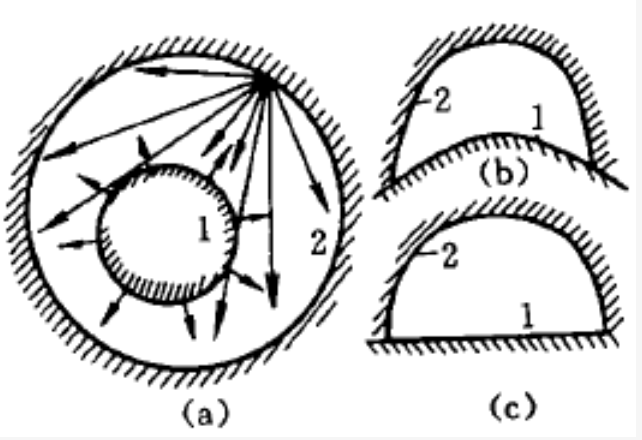
\includegraphics[height=1cm, width=0.3\linewidth]{fig/1.png}
 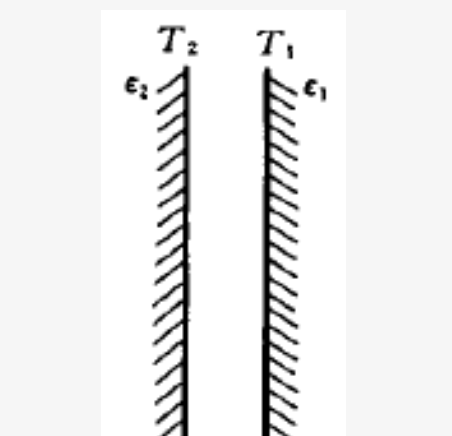
\includegraphics[height=1cm, width=0.3\linewidth]{fig/2.png}
 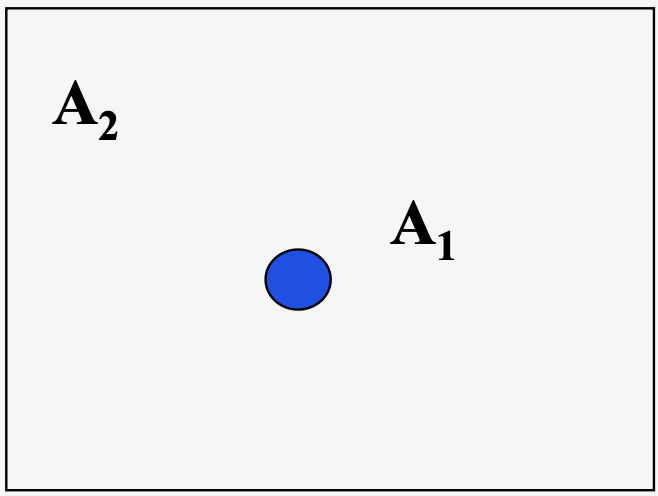
\includegraphics[height=1cm, width=0.3\linewidth]{fig/3.png}\par
}

\vspace{0.5em}

1. 表面 1 为非凹面，\m{X_{1, 1} = 0}，\m{X_{1, 2} = 1}
$$\Phi_{1, 2} = \frac{A_1(E_{b1} - E_{b2})}{\frac{1}{\varepsilon_1} + \frac{A_1}{A_2} \left( \frac{1}{\varepsilon_2} - 1 \right)}$$

2. \m{X_{1, 2} = 1}，表面积 \m{A_1 \approx A_2} 且无限靠近
$$\Phi_{1, 2} = \frac{A_1(E_{b1} - E_{b2})}{\frac{1}{\varepsilon_1} + \frac{1}{\varepsilon_2} - 1}$$

3. \m{X_{1, 2} = 1}，表面积 \m{A_1 \ll A_2}
$$\Phi_{1, 2} = \varepsilon_1 A_1 (E_{b1} - E_{b2})$$

\vspace{0.5em}

(原谅这里公式字母表达不规范，毕竟是 Cheat Sheet，手敲 \LaTeX)

\end{cheatsheet}
\end{document}
